Given a sentence $\mathcal{S}$ as a $n$-length sequence of tokens, $\mathcal{S} = \langle w_1, w_2 \ldots w_n \rangle$, the goal of this module is to output a list of spans (mention tuples) $\langle s, e\rangle$ where $s \in [1, n]$ is the \textit{start} index, $e \in [1, n]$ is the \textit{end} index. Note that the mention tuples are not associated with an entity type. 

We formulate this as a QA task and train a model to extract all required mention spans from a given sentence. Since the goal is to detect only the spans irrespective of their entity type, we use one generic query statement ``\textit{Extract important entity spans from the following text}'' and prefix this with the given sentence before feeding to the model. The model outputs \texttt{B}, \texttt{I}, \texttt{O} or \texttt{E} labels for each token representing the span using \texttt{BIOE} scheme. Figure \ref{fig:framework} shows an example sentence processed by this module.

The \textit{Span Detection Module} must ensure that it identifies mention spans with accurate boundaries. This is because \textit{Span Classification Module} just assigns an entity type to the span. It neither ignores the span nor adjusts its boundaries. In fact, inaccurate mention boundaries could lead to sub-optimal predictions. For example, \textit{Apple} is a \texttt{Fruit}, while \textit{Apple Inc} is an \texttt{Org}.

Many domain specific terms occur rarely and may not have a good semantic representation in the underlying BERT model. However they may have similarities and shared patterns at character-level (for example, chemical formulas). \cite{boukkouri2020characterbert} propose a character-level CNN layer instead of the WordPiece tokenizer at the input stage to the BERT model to better capture such terms. Motivated by this design, we explicitly model character sequences and intrinsic patterns within terms as additional features which are fed to the model along with BERT output.
 
\subsubsection{Character Modeling} Each token output from WordPiece Tokenizer is passed to BERT and simultaneously to five one-dimensional CNNs with kernel sizes of $1$ to $5$, each having $16$ input and $16$ output channels. Each character of the token is indexed and mapped to a $50$-dimensional embedding. Character-level outputs from the CNN are max-pooled to get a token-level representation. Outputs from multiple CNNs are concatenated and passed through a linear layer with ReLU activation to get overall $768$-dimensional feature vector.
    
\subsubsection{Pattern Modeling} Each token output from WordPiece Tokenizer is converted to a pattern encoding. This is done to group together rare tokens which share similarities. The encoding is created by mapping all uppercase letters to \texttt{U}, lowercase to \texttt{L} and digits to \texttt{D}. These are then fed to a Char-CNN (similar to the one above) and then to a bidirectional LSTM with $256$ hidden dimensions to get a contextual pattern feature vector.
    
Finally, these character and pattern features are concatenated with the BERT outputs for the token and fed to a final classifier linear layer. 
    
% This character and pattern modeling is a customization over the vanilla BERT model, adapted to learn better mention boundaries. \comment{maybe? we could say this customization is more effective when done on span detection rather than full NER BERT? :} Note that we could do this because we split our task up into simpler sub-tasks and decided to tackle them one at a time. \comment{can give table in appendix to show some example boundary detection issues motivating char-pattern modeling}

\begin{figure}[h!]
    \centering
    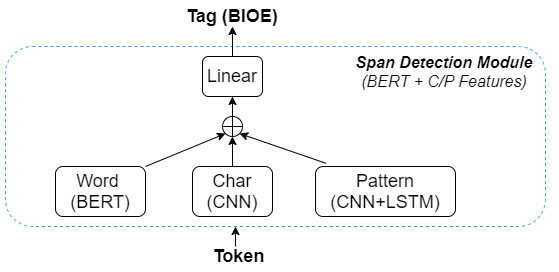
\includegraphics[width=\linewidth]{span_det6.png}
    \caption{Span Detection Module (token-level schematic)}
    \label{fig:span_detection}
\end{figure}
